\documentclass[11pt,a4paper]{article}
\usepackage[T1]{fontenc}
\usepackage[utf8]{inputenc}
\usepackage{lmodern}
\usepackage[margin=24mm,headheight=15pt]{geometry}
\usepackage{amsmath,amssymb,amsthm,mathtools}
\usepackage{microtype,graphicx,booktabs,array,tabularx}
\usepackage[dvipsnames]{xcolor}
\usepackage{enumitem,fancyhdr}
\usepackage{hyperref}
\usepackage{bookmark}
\usepackage{xurl}
\hypersetup{colorlinks=true,linkcolor=MidnightBlue,citecolor=MidnightBlue,urlcolor=MidnightBlue,
 pdftitle={Cubic gap energy for one-sided prime sampling},
 pdfauthor={ChatGPT research report prepared for Vladimir Reshetnikov}}
\urlstyle{same}
\setlength{\emergencystretch}{2em}
\setlength{\parskip}{3pt}
\setlength{\parindent}{0pt}
\setlist{itemsep=3pt,topsep=4pt}
\newtheorem{theorem}{Theorem}[section]
\newtheorem{lemma}[theorem]{Lemma}
\newtheorem{proposition}[theorem]{Proposition}
\newtheorem{corollary}[theorem]{Corollary}
\theoremstyle{definition}
\newtheorem{definition}[theorem]{Definition}
\theoremstyle{remark}
\newtheorem{remark}[theorem]{Remark}
\numberwithin{equation}{section}
\newcommand{\Rea}{\operatorname{Re}}
\newcommand{\Res}{\operatorname{Res}}
\newcommand{\pospart}[1]{\left(#1\right)_{+}}
\pagestyle{fancy}
\fancyhf{}
\fancyhead[L]{\small Cubic gap energy and prime sampling}
\fancyhead[R]{\small Research report / 26 November 2026}
\fancyfoot[C]{\thepage}
\renewcommand{\headrulewidth}{0.3pt}

\begin{document}
\hypersetup{pageanchor=false}
\begin{titlepage}
\vspace*{10mm}
{\color{MidnightBlue}\large MATHEMATICAL RESEARCH REPORT\par}
\vspace{9mm}
{\Huge\bfseries Cubic gap energy for one-sided prime sampling\par}
\vspace{7mm}
{\Large Irregular observations, a sharp density-one obstruction,\par
and consequences for RH and Dirichlet GRH\par}
\vspace{12mm}
{\large Prepared for Vladimir Reshetnikov\par}
{\large 26 November 2026\par}
\vspace{10mm}
\hrule
\vspace{6mm}
\textbf{Main result.} A summable cubic cost for sample gaps, together
with a weighted budget for upper sample values, suffices to exclude
Mellin poles. The criterion accommodates isolated gaps substantially
larger than a uniform mesh permits.

\textbf{Sharpness.} We construct positive coefficients bounded by four
whose smoothed remainder is zero at a set of integers of natural
density one, while its transform has prescribed nonreal poles and no
real poles. This proves a sharp \(5/6\) exponent for geometrically
separated exceptional gaps at the RH scale.

\textbf{Sources.} The readable \texttt{lsernau/grh-lean} development,
and the Riemann hypothesis overview, followed through to the relevant
analytic source files and mathematical antecedents. The inspected commit is
\begin{center}\small\texttt{72fead102f663d5c7a407964a13dc0cf9d977207}\end{center}

\textbf{Status.} Complete human-readable proofs and reproducible
symbolic and numerical checks are supplied. The new statements have
not been formalized in Lean. The repository was inspected at source
level; its full build and independent kernel checks were not repeated.
The novelty claim is restricted to the exact results identified below
and is not a guarantee of worldwide priority.
\vfill
{\small Upstream excerpts retain their original attribution and
Apache-2.0 notices. This paper is an independent research derivation.}
\end{titlepage}
\pagenumbering{arabic}
\hypersetup{pageanchor=true}

\begin{abstract}
For nonnegative coefficients \(a_n\), consider
\(R(x)=\sum_{n\leq x}a_n(1/n-1/x)-A\log x-B\), with \(A\geq0\).
At logarithmic sample times \(t_j\), write \(h_j=t_{j+1}-t_j\), and
suppose \(R(e^{t_j})\leq b_j\), where \(b_j\geq0\). We prove that
summability, for every \(\sigma>\beta\), of
\[
 \sum_j e^{(1-\sigma)t_j}
       \bigl[h_j(b_j+b_{j+1})+A h_j^3\bigr]
\]
forces the meromorphic Mellin transform of \(R\) to be holomorphic in
\(\Rea s>\beta\), provided its real poles there are simple with
nonnegative residues. The proof combines exact convex interpolation
with the classical Landau principle. The contribution is the discrete
criterion and its sharpness, not the Landau principle itself.

For the smoothed Mangoldt remainder, this yields an RH-equivalent
positive-part sampling criterion on every admissible mesh. Exact
power grids \(x_j=j^p\) are admissible precisely when
\(p\leq2/(1-\beta)\). At \(\beta=1/2\), geometrically separated holes
of size \(X^{5/6}\) are also admissible. An explicit family of bounded
positive real coefficients has zero readings on a density-one set,
exceptional gaps of size \(X^{(2+\beta)/3}\), and simple poles at
\(\beta+(2m+1)\pi i\), each of residue \(1/140\). Its cubic energy
has abscissa exactly \(\beta\). We also state the corresponding
Dirichlet criterion, allowing the observation grid to depend on the
quadratic twist selected in the upstream proof.
\end{abstract}

\tableofcontents
\newpage

\section{What is proved here, and what comes from the sources}
\label{sec:status}

The supplied sources now describe a formal proof of RH and of GRH for
Dirichlet \(L\)-functions. The repository's exact exported scope is
important: it includes all positive moduli and imprimitive Dirichlet
characters, but does not by itself assert GRH for arbitrary Artin,
automorphic, or number-field \(L\)-functions
\cite{repo,statements,main,wikipedia}. This report accepts those
statements as the upstream result while distinguishing a source audit
from an independent replay of the complete formal proof.

The present argument studies an analytic interface exposed by that
proof: nonnegative prime weights give convexity, and a sufficiently
small \emph{upper} bound on a smoothed prime remainder excludes poles
of its transform. We replace pointwise control between observations
by a summable cost for the entire observation mesh. The resulting
criterion is unconditional as an abstract theorem about positive
coefficients. Its zeta specialization is an equivalence, so its proof
does not need to assume RH in advance.

\subsection{A pinned source audit}

The inspected revision is
\begin{center}
\texttt{72fead102f663d5c7a407964a13dc0cf9d977207},
\end{center}
committed on 25 November 2026. The selected snapshots and their hashes
are supplied in the archive. The readable project specifies Lean
\texttt{v4.35.0} and Mathlib revision beginning \texttt{56a005855ea1}.
Its README reports compilation without proof placeholders in the built
development, axiom output restricted to \texttt{propext},
\texttt{Classical.choice}, and \texttt{Quot.sound}, and independent
checker acceptance. Those are \emph{upstream-reported} checks; they
were not rerun here \cite{repo,readable}.
The original formal proof is also covered by the joint Lean FRO and
Mathlib verification statement, which reports statement comparison
and independent proof checking \cite{leanverification}.

The file \texttt{Statements.lean} fixes the external propositions using
Mathlib, and \texttt{Main.lean} exports the following five statements:
\begin{center}
\begin{tabularx}{\linewidth}{@{}p{0.26\linewidth}X@{}}
\toprule
Export & Mathematical scope\\
\midrule
RH & Mathlib's \texttt{RiemannHypothesis}.\\
Zeta zeros & Apart from trivial negative even zeros and the explicitly
excepted point \(1\), a zeta zero has real part \(1/2\).\\
Dirichlet nonvanishing & Every Dirichlet \(L(s,\chi)\) is nonzero for
\(\Rea s>1/2\), with the principal pole excepted.\\
Dirichlet zeros & A zero in \(0<\Rea s<1\) has real part \(1/2\).\\
Primitive specialization & The preceding zero statement for primitive
characters.\\
\bottomrule
\end{tabularx}
\end{center}

The main argument compares upper and lower bounds for the same
lattice quantity. Short integral forms give an upper bound, a
second-moment argument supplies enough independent forms, and
theta-lift determinants and the product formula give a lower bound.
Their common main term cancels, leaving a one-sided prime remainder
estimate. In the source notation,
\[
 m\,\mathrm{totalRemainder}\leq f a(\log b)^5.
\]
The number of lifts satisfies \(m\asymp\sqrt{x}\); this is where the
square-root scale enters the final comparison \cite{guide,comparison}.
The construction involves CM fields, unitary theta lifts, integral
lattices, and anticyclotomic twists. The present paper does not
reconstruct these arithmetic inputs.

The directly reused interface lies in
\texttt{PrimeError.lean} and \texttt{Criterion.lean}, together with
the library file \nolinkurl{Lib/Analytic/Landau.lean}. They pass from positive prime
weights to a polar transform and then use an upper bound alone to
remove its poles \cite{primeerror,criterion,landaucode}.

\subsection{Novelty boundary}

Convex interpolation, Landau's theorem, and RH criteria based on
one-sided smoothed prime sums are established inputs. In particular,
Setiawan's preprint already gives a maximum-gap sampling theorem and a
fourth-power criterion \cite{setiawan}. We do not claim either of
those results as new. The original Alp\"oge development and its
expositions also treat weighted upper majorants on late intervals;
our global weighted-integrability argument is an elementary instance
of the same classical analytic principle \cite{rubinstein,odesky}.

The candidate contribution is the precise \emph{discrete cubic
mesh-energy criterion}, its treatment of irregular and omitted
observations, and the matching density-one counterexample with bounded
positive coefficients, no real transform poles, and explicit nonreal
residues. Targeted searches did not locate this exact combination.
That is a limited novelty assessment, not a proof of historical
priority. All the mathematical assertions in the main theorems are
proved below irrespective of their ultimate priority status.

\section{The cubic sampling theorem}
\label{sec:main}

For a real number \(u\), write \(u_+=\max(u,0)\). Let \(a_n\geq0\),
\(A\geq0\), and \(B\in\mathbb R\), and define, for \(x\geq1\),
\begin{equation}
 S(x)=\sum_{n\leq x}a_n\left(\frac1n-\frac1x\right),
 \qquad R(x)=S(x)-A\log x-B.
 \label{eq:remainder}
\end{equation}
The sum is finite on every bounded interval. Its smoothing factor
vanishes at \(n=x\), so no endpoint half-weight convention is needed.
Set \(E(t)=R(e^t)\), for \(t\geq0\), and use the transform
\begin{equation}
 P(s)=\int_1^\infty R(x)x^{-s}\,dx
     =\int_0^\infty E(t)e^{(1-s)t}\,dt.
 \label{eq:transform}
\end{equation}

\begin{theorem}[Cubic sampling criterion]
\label{thm:cubic}
Fix \(\beta<1\). Assume that \eqref{eq:transform} converges absolutely
in some right half-plane and has a meromorphic continuation to
\(\Rea s>\beta\). Assume every real pole in that half-plane is simple
and has nonnegative residue.

Let \(0\leq t_1<t_2<\cdots\) with \(t_j\to\infty\), put
\(h_j=t_{j+1}-t_j\), and assume \(h_j\leq1\) eventually. Suppose
\(b_j\geq0\) and \(E(t_j)\leq b_j\). If, for every real
\(\sigma>\beta\),
\begin{equation}
 \mathcal B_\sigma
 :=\sum_j e^{(1-\sigma)t_j}
       \left[h_j(b_j+b_{j+1})+A h_j^3\right]<\infty,
 \label{eq:budget}
\end{equation}
then \(P\) is holomorphic throughout \(\Rea s>\beta\).
\end{theorem}

The pole condition is automatic if \(P\) is regular on the real axis.
Only \emph{real} poles are restricted in the hypothesis; nonreal poles
may have arbitrary finite orders. When \(A>0\), the condition
\(h_j\leq1\) eventually already follows from
\eqref{eq:budget}: choose \(\beta<\sigma<1\), and observe that
\(e^{(1-\sigma)t_j}h_j^3\to0\). It is stated explicitly to cover
\(A=0\) without a separate convention.

The theorem does not impose a common pointwise power bound on the
readings. A large upper value is allowed if its weighted contribution
to \eqref{eq:budget} remains summable. Likewise, a few long gaps can be
less costly than many moderately long gaps.

\subsection{Exact interpolation}

\begin{lemma}[The gap envelope]
\label{lem:envelope}
For \(0\leq y\leq h\), define
\[
 \theta_h(y)=\frac{1-e^{-y}}{1-e^{-h}},\qquad
 J_h(y)=h\theta_h(y)-y.
\]
Then \(J_h\geq0\), and
\begin{equation}
 E(t+y)\leq(1-\theta_h(y))E(t)+\theta_h(y)E(t+h)
              +A J_h(y).
 \label{eq:envelope}
\end{equation}
Moreover,
\begin{equation}
 I(h):=\int_0^hJ_h(y)\,dy
   =\frac{h^2}{1-e^{-h}}-h-\frac{h^2}{2}
   =\frac{h^3}{12}-\frac{h^5}{720}+O(h^7).
 \label{eq:exactcost}
\end{equation}
For \(0<h\leq1\),
\begin{equation}
 \frac{e^{-1}h^3}{12}\leq I(h)\leq\frac{eh^3}{12}.
 \label{eq:cubiccost}
\end{equation}
\end{lemma}

\begin{proof}
Positivity of the coefficients makes
\[
 T(x):=xS(x)=\sum_{n\geq1}a_n\left(\frac xn-1\right)_+
\]
convex. Equivalently, \(S(1/u)=\sum_n a_n(1/n-u)_+\) is convex in
\(u>0\). The identity
\[
 e^{-(t+y)}=(1-\theta_h(y))e^{-t}
                     +\theta_h(y)e^{-(t+h)}
\]
therefore bounds \(S(e^{t+y})\) by the corresponding endpoint chord.
Subtracting \(A(t+y)+B\) gives \eqref{eq:envelope}; the constant
\(B\) cancels exactly.

The function \(J_h\) is concave, with zero values at both endpoints,
because
\[
 -J_h''(y)=\frac{h e^{-y}}{1-e^{-h}}>0.
\]
Thus it is nonnegative. Integration gives the exact expression in
\eqref{eq:exactcost}; its expansion follows from the Taylor expansion
of \((1-e^{-h})^{-1}\). If \(h\leq1\), then
\(e^{-1}\leq-J_h''\leq e\). Comparison with the parabolas
\(e^{-1}y(h-y)/2\) and \(ey(h-y)/2\), followed by integration,
proves \eqref{eq:cubiccost}.
\end{proof}

The height of a single gap envelope is of order \(h^2\), but its
\emph{integrated} cost is of order \(h^3\). This extra factor of gap
length is the reason irregular meshes can outperform a criterion that
uses only their largest gap.

\begin{figure}[htbp]
\centering
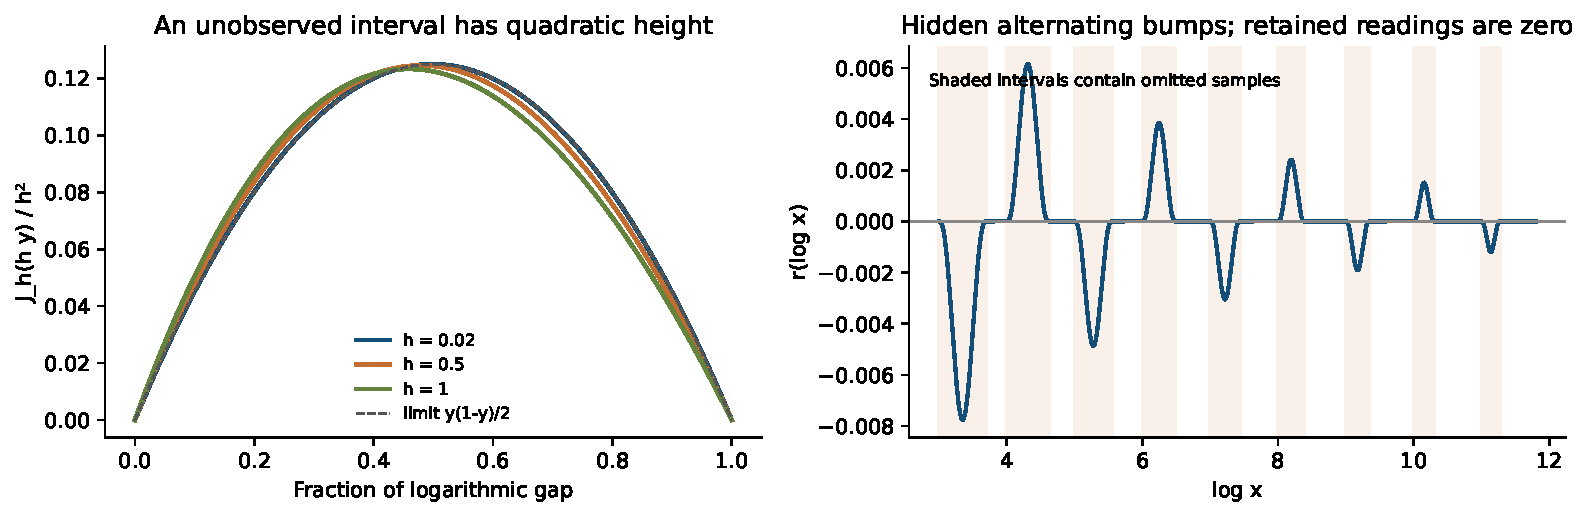
\includegraphics[width=\linewidth]{figures/cubic_mechanism.pdf}
\caption{The interpolation mechanism and its cumulative cost.
The exact gap integral has leading term \(h^3/12\); the theorem sums
these costs with the Mellin weight. The figure is illustrative, while
Lemma~\ref{lem:envelope} gives the exact formula and bounds.}
\label{fig:cubic}
\end{figure}

\subsection{From the discrete budget to a one-sided majorant}

On each sufficiently late interval \([t_j,t_{j+1}]\), define
\[
 H(t_j+y)=(1-\theta_{h_j}(y))b_j
            +\theta_{h_j}(y)b_{j+1}+A J_{h_j}(y).
\]
Lemma~\ref{lem:envelope} gives \(H\geq E\), and \(H\geq0\).
For every fixed real \(\sigma\), the factor
\(e^{(1-\sigma)y}\) varies by at most \(e^{|1-\sigma|}\) on a gap of
length at most one. Hence
\begin{align}
 \int_{t_j}^{t_{j+1}}H(t)e^{(1-\sigma)t}\,dt
 &\leq e^{|1-\sigma|}e^{(1-\sigma)t_j}
       \left[h_j(b_j+b_{j+1})+\frac{Ae}{12}h_j^3\right]\notag\\
 &\leq e^{|1-\sigma|}e^{(1-\sigma)t_j}
       \left[h_j(b_j+b_{j+1})+A h_j^3\right].
 \label{eq:majorantcost}
\end{align}
Thus \eqref{eq:budget} makes the transform of \(H\) holomorphic for
\(\Rea s>\beta\). Local uniform convergence, and the same estimate
with a slightly smaller real part, justify differentiation under the
integral on compact subsets.

\subsection{The Landau comparison, with signs made explicit}

\begin{lemma}[Landau's real-boundary principle]
\label{lem:landau}
Let \(V(t)\geq0\) be locally integrable on a half-line. If
\(Q(s)=\int V(t)e^{(1-s)t}\,dt\) has finite convergence abscissa
\(c\), then \(Q\) cannot be holomorphic in a neighborhood of the real
point \(c\).
\end{lemma}

\begin{proof}
Suppose \(Q\) is holomorphic on \(|s-c|<r\). Choose
\(s_0=c+r/4\). Its Taylor series converges at \(s_0-r/2<c\), since
the disk centered at \(s_0\) of radius \(3r/4\) lies in the given
disk. Differentiation at \(s_0>c\) gives
\[
 (-1)^n Q^{(n)}(s_0)=\int t^nV(t)e^{(1-s_0)t}\,dt\geq0.
\]
One may first start the half-line at a nonnegative point, changing
only an entire function. Monotone convergence applied to the
nonnegative Taylor terms then shows that
\[
 \int V(t)e^{(1-s_0+r/2)t}\,dt
 =\sum_{n\geq0}\frac{(r/2)^n}{n!}
             \int t^nV(t)e^{(1-s_0)t}\,dt<\infty.
\]
This is convergence to the left of \(c\), a contradiction.
\end{proof}

\begin{proof}[Proof of Theorem~\ref{thm:cubic}]
Discard a finite initial interval, which changes transforms by entire
functions, and use the majorant \(H\) above. The function
\(V=H-E\) is nonnegative. Its transform converges in a right
half-plane, since the transforms of both \(H\) and \(E\) do so.
Write \(c\) for its convergence abscissa.

If \(c>\beta\), then the identity
\[
 Q(s)=\widehat H(s)-P(s)+\text{an entire function}
\]
continues \(Q\) meromorphically across the real point \(c\).
Lemma~\ref{lem:landau} says that this point is singular. But its only
possible singularity is a simple pole with residue equal to minus the
residue of \(P\), and therefore nonpositive. A strictly negative
residue would force \(Q(s)\to-\infty\) as real \(s\downarrow c\),
contrary to \(Q(s)\geq0\). A zero residue is removable, again a
contradiction. Thus \(c\leq\beta\). Both \(Q\) and
\(\widehat H\) are now holomorphic for \(\Rea s>\beta\), so their
difference gives the same conclusion for \(P\).
\end{proof}

\begin{remark}[Observational error and missing readings]
If a reported value \(y_j\) has a certified upper error
\(\varepsilon_j\geq0\), meaning \(E(t_j)\leq y_j+\varepsilon_j\),
one may use \(b_j=(y_j+\varepsilon_j)_+\). The theorem then charges
exactly the sample budget in \eqref{eq:budget}. Discarding readings
merges adjacent gaps and changes their cubic cost. These are
deterministic consequences; no probabilistic noise model is needed.
They do not turn finitely many numerical observations into a proof of
an infinite summability condition.
\end{remark}

\section{The zeta function and an RH-equivalent sampling condition}
\label{sec:zeta}

Let \(\Lambda\) denote the von Mangoldt function and \(\gamma_E\)
Euler's constant. The appropriate normalized remainder is
\begin{equation}
 R_\zeta(x)=\sum_{n\leq x}\Lambda(n)
      \left(\frac1n-\frac1x\right)-\log x+1+\gamma_E.
 \label{eq:zetaremainder}
\end{equation}
In the notation of \eqref{eq:remainder}, this is \(A=1\) and
\(B=-1-\gamma_E\). The additive constant matters: an incorrect
normalization leaves a pole at \(s=1\).

For \(\Rea s>1\), termwise integration of the absolutely convergent
Dirichlet series gives
\begin{equation}
 P_\zeta(s)=
 \frac{-\zeta'(s)/\zeta(s)}{s(s-1)}
 -\frac1{(s-1)^2}+\frac{1+\gamma_E}{s-1}.
 \label{eq:zetatransform}
\end{equation}
Indeed,
\(\int_n^\infty(1/n-1/x)x^{-s}\,dx=n^{-s}/[s(s-1)]\).
Since
\(-\zeta'/\zeta=1/(s-1)-\gamma_E+O(s-1)\), both polar terms at
\(s=1\) cancel. If \(\rho\) is a nontrivial zero of multiplicity
\(m_\rho\), the corresponding residue is
\begin{equation}
 \Res_{s=\rho}P_\zeta(s)
   =\frac{m_\rho}{\rho(1-\rho)}\ne0.
 \label{eq:zetaresidue}
\end{equation}
These standard smoothed identities are also exposed in the sources
\cite{primeerror,rubinstein}.

There are no zeta zeros on the positive real axis. For \(s>1\) this
follows from its positive Dirichlet series. For \(0<s<1\), the
alternating eta series is positive by grouping consecutive terms,
whereas \(1-2^{1-s}<0\), so
\(\zeta(s)=\eta(s)/(1-2^{1-s})\ne0\). Thus \(P_\zeta\) is
regular on the positive real axis.

\begin{definition}[Admissible mesh at \(\beta\)]
A mesh \(0\leq t_j\uparrow\infty\), with \(h_j=t_{j+1}-t_j\), is
admissible at \(\beta<1\) if
\[
 \sum_j e^{(1-\sigma)t_j}h_j^3<\infty
 \quad\text{for every }\sigma>\beta.
\]
This condition forces \(h_j\to0\).
\end{definition}

\begin{theorem}[RH from upper readings on an admissible mesh]
\label{thm:RH-equivalence}
Fix any mesh admissible at \(1/2\), and set
\(b_j=(R_\zeta(e^{t_j}))_+\). Then RH is equivalent to
\begin{equation}
 \sum_j e^{(1-\sigma)t_j}h_j(b_j+b_{j+1})<\infty
 \quad\text{for every }\sigma>1/2.
 \label{eq:RHsamples}
\end{equation}
\end{theorem}

\begin{proof}
Suppose first that \eqref{eq:RHsamples} holds. The cubic part of the
budget is finite by admissibility. Theorem~\ref{thm:cubic},
\eqref{eq:zetatransform}, and real-axis regularity make
\(P_\zeta\) holomorphic for \(\Rea s>1/2\). Equation
\eqref{eq:zetaresidue} then excludes every zeta zero to the right of
that line. The functional equation reflects any zero to its left to
one on its right, proving RH.

Conversely assume RH. The classical RH estimate
\(\psi(x)-x=O(x^{1/2}\log^2x)\), where
\(\psi(x)=\sum_{n\leq x}\Lambda(n)\), gives
\begin{equation}
 R_\zeta(x)=-\int_x^\infty\frac{\psi(u)-u}{u^2}\,du
       =O(x^{-1/2}\log^2x).
 \label{eq:RHbound}
\end{equation}
The integral identity follows by integration of the almost-everywhere
identity \(R_\zeta'(x)=(\psi(x)-x)/x^2\); the remainder is locally
absolutely continuous.
To check its integration constant, the displayed RH estimate implies
that \(S(x)-\log x=\int_1^x(\psi(u)-u)u^{-2}\,du\) has a finite
limit \(C\). The elementary Abel limit identifies \(C\) with the
residue at \(s=1\) of the transform of \(S-\log x\).
The Laurent expansion used above gives \(C=-1-\gamma_E\), so
\(R_\zeta(x)\to0\). The identity also follows from the smoothed
explicit formula \cite{mv,rubinstein}.
Hence for \(\sigma>1/2\), the summand in
\eqref{eq:RHsamples} is at most a constant times
\(h_j e^{-(\sigma-1/2)t_j}(1+t_j)^2\). Since \(h_j\leq1\)
eventually, its sum is bounded by a constant multiple of the
convergent integral
\(\int_0^\infty e^{-(\sigma-1/2)t}(1+t)^2\,dt\).
\end{proof}

This theorem gives a condition on upper readings only; negative values
incur no sample cost. A convenient sufficient condition is
\(R_\zeta(e^{t_j})\leq C e^{-t_j/2}(1+t_j)^M\) for some fixed
\(C,M\), provided the mesh is admissible. The equivalence remains an
infinite theorem, not a finite computational certificate.

\section{Which meshes are permitted?}
\label{sec:meshes}

\subsection{Exact power grids}

\begin{proposition}
\label{prop:powergrid}
For the exact grid \(x_j=j^p\), with \(p>0\), admissibility at
\(\beta<1\) holds if and only if
\[
 p\leq\frac2{1-\beta}.
\]
\end{proposition}

\begin{proof}
Here \(t_j=p\log j\) and
\(h_j=p\log(1+1/j)\sim p/j\). Thus the cubic series at \(\sigma\)
is comparable to
\(\sum_j j^{p(1-\sigma)-3}\), which converges exactly when
\(p(1-\sigma)<2\). Requiring this for every \(\sigma>\beta\)
is equivalent to the displayed condition, including equality.
\end{proof}

At \(\beta=1/2\), the endpoint is \(p=4\). Fourth-power sampling
itself is an antecedent, as noted in Section~\ref{sec:status}. The
statement concerns the exact grid, or a mesh with comparably controlled
local gaps. The asymptotic relation \(x_j\sim j^p\) alone is not
enough: it can conceal exceptional large gaps.

\subsection{Geometrically separated missing blocks}

Start with all positive integers as potential samples. Near each
\(X_k=e^k\), omit a block of length \(O(X_k^\alpha)\), where
\(0<\alpha<1\), allowing only a bounded number of such blocks in
each multiplicative shell. An exceptional logarithmic gap is
\(O(e^{-(1-\alpha)k})\). Its cubic contribution is therefore
\[
 O\left(e^{(3\alpha-2-\sigma)k}\right).
\]
The ordinary unit gaps contribute at most
\(\sum_n O(n^{-2-\sigma})\). Consequently the resulting mesh is
admissible whenever \(-1<\beta<1\) and \(\beta\geq3\alpha-2\).

In particular, one can omit geometrically separated blocks of size
\(X^{5/6}\) and still use Theorem~\ref{thm:RH-equivalence}. Such gaps
are much larger than the \(X^{3/4}\) scale of the uniform quartic
mesh. There is no contradiction: a uniform mesh repeats its largest
cost throughout each shell, whereas the present mesh pays for only a
bounded number of exceptional gaps there.

More generally, if a shell near \(X\) contains
\(O(X^d)\) gaps of size \(O(X^\alpha)\), their total cubic cost is
\(O(X^{d+3\alpha-2-\sigma})\). Summation over geometric shells
therefore yields the sufficient exponent \(\beta\geq d+3\alpha-2\).
For a uniform mesh, \(d=1-\alpha\), recovering
\(\beta\geq2\alpha-1\). This calculation describes a tradeoff
between the number and the size of omitted intervals, rather than a
bound on their size alone.

\section{A Dirichlet version with twist-dependent grids}
\label{sec:Dirichlet}

The repository's positive coefficients are, for suitable \(q,d\),
\[
 \lambda_{q,d}(n)=\mathbf1_{n\equiv1\ (\mathrm{mod}\ q)}
                  \Lambda(n)\bigl(1-\chi_d(n)\bigr)\geq0,
\]
where \(\chi_d\) is the quadratic character attached to the selected
prime \(d\). It uses the normalized remainder
\begin{equation}
 R_{q,d}(x)=\sum_{n\leq x}\lambda_{q,d}(n)
       \left(\frac1n-\frac1x\right)
       -\frac{\log x}{\varphi(q)}-c_{q,d}.
 \label{eq:Dirichletremainder}
\end{equation}
The constant \(c_{q,d}\) is the upstream normalization making the
remainder tend to zero. The transform is meromorphic for \(\Rea s>0\).
Away from \(1\), its residue is
\begin{equation}
 \frac{\displaystyle\sum_{\chi\bmod q}
       \operatorname{ord}_s L^*(\chi)
       -\displaystyle\sum_{\chi\bmod q}
       \operatorname{ord}_s L^*(\chi\chi_d)}
      {\varphi(q)s(1-s)},
 \label{eq:Dirichletresidue}
\end{equation}
where \(L^*\) denotes the entire function obtained by removing a
principal pole \cite{primeerror}.

A key arithmetic input is the quadratic-twist selection theorem used
in \texttt{Criterion.lean}: given a proposed zero and a suitable
congruence class for \(d\), one can choose a prime \(d\) in that
class such that all the twisted functions in
\eqref{eq:Dirichletresidue} are zero-free in the required finite
rectangle. This covers the target zero and every possible relevant
real zero. It makes the real residues nonnegative and the residue at
the target zero nonzero \cite{criterion}.

\begin{corollary}[Cubic sampling after twist selection]
\label{cor:Dirichlet}
Fix \(1/2<\beta<1\), a positive multiple \(q\) of \(8\), and a
class \(d_0\) coprime to \(q\) with \(d_0\equiv7\pmod8\), in the
setting of the upstream criterion. Suppose that for every prime
\(d\equiv d_0\pmod q\) there are a mesh
\(t_j^{(d)}\uparrow\infty\) and numbers \(b_j^{(d)}\geq0\) such that
\[
 R_{q,d}(e^{t_j^{(d)}})\leq b_j^{(d)}
\]
and, for every \(\sigma>\beta\),
\[
 \sum_j e^{(1-\sigma)t_j^{(d)}}
 \left[h_j^{(d)}(b_j^{(d)}+b_{j+1}^{(d)})
             +\frac{(h_j^{(d)})^3}{\varphi(q)}\right]<\infty.
\]
Then every Dirichlet \(L(s,\chi)\) modulo \(q\) is nonzero for
\(\Rea s>\beta\), with the principal pole excepted.
\end{corollary}

\begin{proof}
If a zero \(\rho\) existed, choose the prime \(d\) furnished by the
upstream twist-selection result. For this single \(d\), the transform
has nonnegative real residues and a nonzero residue at \(\rho\).
Apply Theorem~\ref{thm:cubic} with \(A=1/\varphi(q)\) on its assigned
mesh. The transform is holomorphic to the right of \(\beta\), a
contradiction.
\end{proof}

No common mesh or uniform bound on the budgets across different
\(d\) is required: the contradiction uses only the selected twist.
The quantifier over every eligible prime \(d\), however, is essential
unless one separately knows which twist can be selected. Taking
\(\beta\downarrow1/2\), together with the standard functional
equation, gives the corresponding Dirichlet GRH criterion. This
corollary reuses the upstream arithmetic selection theorem; it does
not supply a new proof of that theorem or extend its scope to general
nonabelian \(L\)-functions.

% Standalone section fragment; assumes amsmath, amssymb, amsthm.
\section{A sharp obstruction with almost every integer sampled}
\label{sec:density-one-obstruction}

The cubic gap cost cannot be improved using only positivity of the
coefficients and regularity of the transform on the real axis. The
following construction makes this precise. Its coefficients are bounded
positive real numbers; no multiplicativity or Euler product is asserted.

\begin{theorem}[A sharp density-one obstruction]
\label{thm:density-one-obstruction}
Fix $0<\beta<1$, and put $\delta=(1-\beta)/3$. There exist a sequence
$(a_n)_{n\geq1}$ and a set $S\subseteq\mathbb N_{\geq1}$ such that
\begin{enumerate}
\item $0<a_n<4$ for every $n$.
\item The remainder
\[
 R(x)=\sum_{n\leq x}a_n\left(\frac1n-\frac1x\right)-\log x
\]
vanishes at every $n\in S$, and
\[
 \#\bigl([1,X]\cap(\mathbb N\setminus S)\bigr)
       =O_\beta\bigl(X^{(2+\beta)/3}\bigr).
\]
In particular, $S$ has natural density one.
\item The Mellin transform
\[
 \mathcal M(s)=\int_1^\infty R(x)x^{-s}\,dx
\]
has a meromorphic continuation to $\operatorname{Re}s>-1$ with no real
poles. Its rightmost poles are exactly
\[
 s=\beta+(2m+1)\pi i,\qquad m\in\mathbb Z,
\]
and each is simple with residue $1/140$.
\item If $x_1<x_2<\cdots$ enumerate $S$, then
\[
 \sum_n x_n^{1-\sigma}
       \left(\log\frac{x_{n+1}}{x_n}\right)^3<\infty
       \quad\Longleftrightarrow\quad \sigma>\beta.
\]
Apart from gaps of length one, the successive sample gaps occur near
$X_k=e^k$ and have length asymptotic to $X_k^{(2+\beta)/3}$.
\end{enumerate}
\end{theorem}

\begin{proof}
Let $K\geq2$ be an integer. Define the globally $C^2$ function
\[
 \phi(u)=
 \begin{cases}u^3(1-u)^3,&0\leq u\leq1,\\0,&\text{otherwise},\end{cases}
 \qquad h_k=e^{-\delta k},
\]
and put
\[
 r(t)=\sum_{k\geq K}(-1)^k h_k^2
                  \phi\left(\frac{t-k}{h_k}\right),
 \qquad F(x)=x\log x+xr(\log x).
\]
The summands have disjoint supports $[k,k+h_k]$. Their first two
derivatives match zero at the endpoints, so $r$ is $C^2$.

We first verify convexity with explicit constants. Writing
$z=u(1-u)\in[0,1/4]$ gives
\[
 \phi'(u)=3u^2(1-u)^2(1-2u),\qquad
 \phi''(u)=6z(1-5z).
\]
Thus $|\phi'|\leq3/16$ and $|\phi''|\leq3/8$. As $h_k\leq1$ and
the supports are disjoint,
\[
 |r'(t)+r''(t)|\leq\frac9{16}.
\]
Differentiation now yields
\begin{equation}
 \frac7{16x}\leq F''(x)
   =\frac{1+r'(\log x)+r''(\log x)}x
   \leq\frac{25}{16x}.
 \label{eq:obstruction-curvature}
\end{equation}

Define
\[
 a_1=F(2)=2\log2,\qquad
 a_n=n\bigl(F(n+1)-2F(n)+F(n-1)\bigr)\quad(n\geq2).
\]
The tent-kernel identity and \eqref{eq:obstruction-curvature} imply
\[
 \frac7{16}\frac n{n+1}\leq a_n
 =n\int_{n-1}^{n+1}(1-|x-n|)F''(x)\,dx
 \leq\frac{25}{16}\frac n{n-1}\leq\frac{25}8<4
\]
for $n\geq2$. This proves the coefficient bounds.

Let $IF$ denote the linear interpolant of $F$ at the positive integers.
Because $F(1)=0$, telescoping the second differences gives
\[
 IF(x)=a_1(x-1)+\sum_{2\leq n\leq x}\frac{a_n}{n}(x-n),
 \qquad R(x)=\frac{IF(x)}x-\log x.
\]
Convexity gives $IF\geq F$. For $n\leq x\leq n+1$, the usual chord
bound following from \eqref{eq:obstruction-curvature} gives
$IF(x)-F(x)\leq25/(128n)$. Since $n\geq x/2$, we obtain
\begin{equation}
 0\leq R(x)-r(\log x)\leq\frac{25}{64x^2}.
 \label{eq:obstruction-interpolation-error}
\end{equation}

Take
\[
 S=\left\{n\geq1:\log n\notin
              \bigcup_{k\geq K}(k,k+h_k)\right\}.
\]
At every $n\in S$, $r(\log n)=0$ and $IF(n)=F(n)=n\log n$, so
$R(n)=0$ exactly. The deleted integers up to $X$ number at most
\[
 \sum_{K\leq k\leq\log X}
       \left(e^k(e^{h_k}-1)+2\right)
       =O_\beta(X^{1-\delta}),
\]
which proves the density assertion.

It remains to determine the transform, including its real-axis
regularity. Set
\[
 \Phi(z)=\int_0^1\phi(v)e^{zv}\,dv,\qquad
 \mu_j=\int_0^1v^j\phi(v)\,dv
       =\frac6{(j+4)(j+5)(j+6)(j+7)}.
\]
In particular, $\mu_0=1/140$. Changing variables on each support yields,
initially for $\operatorname{Re}s>\beta$,
\[
 \mathcal M_0(s):=\int_0^\infty r(t)e^{(1-s)t}\,dt
 =\sum_{k\geq K}(-1)^k e^{(\beta-s)k}
       \Phi\bigl((1-s)e^{-\delta k}\bigr).
\]
For every positive integer $J$, Taylor expansion gives
\begin{equation}
 \mathcal M_0(s)=
 \sum_{j=0}^{J-1}\frac{\mu_j(1-s)^j}{j!}
       \frac{(-e^{\beta-s-j\delta})^K}
            {1+e^{\beta-s-j\delta}}
       +H_J(s),
 \label{eq:obstruction-continuation}
\end{equation}
where $H_J$ is holomorphic for
$\operatorname{Re}s>\beta-J\delta$. Indeed, the Taylor remainder is
$O(e^{-J\delta k})$, uniformly for $s$ in any fixed compact set.
As $J$ is arbitrary, this provides a meromorphic continuation of
$\mathcal M_0$ to the plane.

The displayed denominators vanish only at
\[
 s=\beta-j\delta+(2m+1)\pi i.
\]
Their derivatives there are $1$, and the corresponding numerators are
$1$. Hence the residue is $\mu_j(1-s)^j/j!$, which is nonzero. Different
$j$ give distinct vertical lines, and no candidate pole is real.
Equation~\eqref{eq:obstruction-interpolation-error} shows that
$\mathcal M-\mathcal M_0$ is holomorphic on
$\operatorname{Re}s>-1$. It therefore preserves every pole in that
half-plane, proving the asserted pole and residue statements.

Finally, the exceptional gap crossing the $k$th support has endpoints
$\lfloor e^k\rfloor$ and $\lceil e^{k+h_k}\rceil$ for all sufficiently
large $k$. Its ordinary length is asymptotic to $e^{(1-\delta)k}$,
and its logarithmic length is $h_k+O(e^{-k})\sim h_k$. Its energy
contribution is consequently asymptotic to
\[
 e^{(1-\sigma)k}h_k^3=e^{(\beta-\sigma)k}.
\]
The sum of these contributions converges exactly for $\sigma>\beta$.
The other gaps join consecutive integers and contribute
$O(n^{-2-\sigma})$, summable when $\sigma>-1$. This proves the final
assertion; when $\sigma\leq-1$, the already divergent exceptional
subseries suffices.
\end{proof}

\begin{corollary}[The cubic power cannot be reduced in cost]
\label{cor:cubic-optimal}
For any \(p>3\), replacing \(h_j^3\) by \(h_j^p\) in
Theorem~\ref{thm:cubic} makes its conclusion false, even for
bounded positive coefficients, zero sample readings, and a transform
with no real poles.
\end{corollary}

\begin{proof}
Use Theorem~\ref{thm:density-one-obstruction}, and denote its
parameter by \(b\in(0,1)\), so \(\delta=(1-b)/3\).
The exceptional \(p\)-power energy converges for
\(\sigma>1-p\delta=b-(p-3)\delta\).
Ordinary unit gaps contribute \(O(n^{1-\sigma-p})\), a convergent
series for \(\sigma>2-p\).
Choose a proposed boundary
\(\beta_0\in(\max(0,b-(p-3)\delta),b)\).
All modified budgets are finite for every \(\sigma>\beta_0\);
the readings vanish, yet the poles on \(\Rea s=b\) remain.
\end{proof}

\begin{corollary}[The exceptional-gap exponent]
At the boundary $\beta=1/2$, geometrically separated gaps of size
$X^{5/6}$ have finite cubic energy at every exponent $\sigma>1/2$.
For every $5/6<\alpha<1$, there is instead an example as in
Theorem~\ref{thm:density-one-obstruction} with gaps of size $X^\alpha$
and undetected nonreal poles of real part $3\alpha-2>1/2$.
\end{corollary}

\begin{proof}
Set $\beta=3\alpha-2$, so $(2+\beta)/3=\alpha$, and apply the theorem.
At the endpoint, the exceptional energy is a geometric series with
ratio $e^{1/2-\sigma}<1$.
\end{proof}

For comparison with Dirichlet-series formulations, boundedness of
$a_n$ gives absolute convergence of $D(s)=\sum a_nn^{-s}$ for
$\operatorname{Re}s>1$, where direct integration gives
\[
 \mathcal M(s)=\frac{D(s)}{s(s-1)}-\frac1{(s-1)^2},
 \qquad D(s)=\frac{s}{s-1}+s(s-1)\mathcal M(s).
\]
Thus the example is also an explicit positive-coefficient Dirichlet
series with a meromorphic continuation and a fully specified rightmost
nonreal pole family after its leading real pole is subtracted.

\section{Verification, formalization, and limits}
\label{sec:verification}

\subsection{Checks supplied with the paper}

The program \texttt{code/verify\_cubic\_energy.py} checks the derivative
identities for the bump, the exact leading residue, the Taylor series
of \(I(h)\), the coefficient construction, and the integer
reconstruction identity. Its recorded run used
\(\beta=0.65\), \(\delta=(1-\beta)/3\), \(K=3\), and the first
\(100{,}000\) coefficients. The minimum and maximum computed
coefficients were approximately \(0.6240670543\) and
\(1.3862943611\). The maximum reconstruction discrepancy was
\(2.67\times10^{-15}\), and \(66{,}956\) of these integer samples
were retained. High-precision quadrature also checked
\eqref{eq:exactcost} at \(h=0.01,0.1,0.5,1\).

These are finite consistency checks. The positivity of all
coefficients, exact vanishing of infinitely many sample values,
meromorphic continuation, pole residues, and energy boundary are
proved analytically in
Theorem~\ref{thm:density-one-obstruction}. Floating-point observations
alone would establish none of those infinite assertions.

The archive includes selected upstream source snapshots, their
attribution and license, and a source audit. It is not a complete
buildable copy of the upstream formalization. Neither this paper's
new theorem nor its counterexample is claimed to have been checked by
the Lean kernel.

\subsection{A concrete formalization plan}

The proof separates into four manageable interfaces.
\begin{enumerate}
\item \textbf{Finite convexity and interpolation.}
Define the positive hinge sum and prove convexity on each compact
interval. Derive \eqref{eq:envelope} using the reciprocal affine
weights, then evaluate \(I(h)\) and prove its two cubic bounds.
These steps require no arithmetic or complex analysis.
\item \textbf{Series-to-integral transfer.}
Construct the nonnegative piecewise envelope on the partition
\([t_j,t_{j+1}]\), establish measurability, and prove
\eqref{eq:majorantcost}. Tonelli's theorem supplies the sum over gaps;
weighted domination yields holomorphy of the transform.
\item \textbf{Landau comparison.}
Generalize the existing eventual exponential-majorant interface to
an integrable majorant. The only additional bridge is
\(\widehat H-P\), the transform of a nonnegative function, followed
by the real-residue sign argument in the proof of
Theorem~\ref{thm:cubic}.
\item \textbf{Arithmetic specialization and sharpness.}
Reuse the upstream prime remainder, polar transform, and twist
selection for Corollary~\ref{cor:Dirichlet}. Separately formalize the
compact polynomial bump, its integer second differences, the
interpolant identity, and the locally uniform geometric-series
continuation. This last branch is an independent analysis construction
and should not import the difficult arithmetic development.
\end{enumerate}

This is a proof outline, not executable Lean source. In particular,
meromorphic continuation and the infinite partition argument are
substantial formal obligations and should not be hidden behind new
axioms or proof placeholders.

\subsection{What the result does and does not establish}

The sampling theorem proves a new sufficient condition in an abstract
positive-coefficient setting and an exact RH-equivalent condition for
a given admissible mesh. Its matching obstruction demonstrates the
limits of that abstract information. The example has bounded positive
\emph{real} weights; it has no asserted Euler product,
multiplicativity, integrality, or prime interpretation. Consequently
it does not show that all stronger prime-specific sampling theorems
are impossible.

The \(5/6\) endpoint describes geometrically separated exceptional
holes. It is not an improved general bound on gaps between primes,
nor a replacement of the uniform \(3/4\) sampling scale. The latter
and fourth-power sampling are explicitly credited as earlier results.
The distinction is quantitative: the criterion measures the sum of
gap costs, and the obstruction matches the abscissa of that sum.

The main mathematical takeaway is therefore precise. For reciprocal
ramp sums with positive coefficients, the correct integrated
observation cost is cubic in logarithmic gap length. The source
proof's one-sided analytic mechanism can use that aggregate cost,
while a density-one family of observations alone cannot prevent a
nonreal pole from hiding in suitably arranged large gaps.

\begin{thebibliography}{99}
\small
\bibitem{repo}
L. Sernau and collaborators,
\emph{GRH for Dirichlet L-functions, in Lean 4}, repository root README,
revision \texttt{72fead102f663d5c7a407964a13dc0cf9d977207},
25 November 2026.
\url{https://github.com/lsernau/grh-lean/blob/72fead102f663d5c7a407964a13dc0cf9d977207/README.md}.

\bibitem{readable}
\emph{grh-lean}, readable-project README, same revision.
\url{https://github.com/lsernau/grh-lean/blob/72fead102f663d5c7a407964a13dc0cf9d977207/grh/README.md}.

\bibitem{statements}
\emph{grh-lean}, \texttt{grh/src/Statements.lean}, same revision.
\url{https://github.com/lsernau/grh-lean/blob/72fead102f663d5c7a407964a13dc0cf9d977207/grh/src/Statements.lean}.

\bibitem{main}
\emph{grh-lean}, \texttt{grh/src/Main.lean}, same revision.
\url{https://github.com/lsernau/grh-lean/blob/72fead102f663d5c7a407964a13dc0cf9d977207/grh/src/Main.lean}.

\bibitem{guide}
\emph{grh-lean}, \texttt{grh/GUIDE.md}, same revision.
\url{https://github.com/lsernau/grh-lean/blob/72fead102f663d5c7a407964a13dc0cf9d977207/grh/GUIDE.md}.

\bibitem{comparison}
\emph{grh-lean}, \texttt{New/Reduction/MainInequality.lean}, same revision.
\url{https://github.com/lsernau/grh-lean/blob/72fead102f663d5c7a407964a13dc0cf9d977207/grh/src/New/Reduction/MainInequality.lean}.

\bibitem{primeerror}
\emph{grh-lean}, \texttt{New/Reduction/Zeros/PrimeError.lean}, same revision.
\url{https://github.com/lsernau/grh-lean/blob/72fead102f663d5c7a407964a13dc0cf9d977207/grh/src/New/Reduction/Zeros/PrimeError.lean}.

\bibitem{criterion}
\emph{grh-lean}, \texttt{New/Reduction/Zeros/Criterion.lean}, same revision.
\url{https://github.com/lsernau/grh-lean/blob/72fead102f663d5c7a407964a13dc0cf9d977207/grh/src/New/Reduction/Zeros/Criterion.lean}.

\bibitem{landaucode}
\emph{grh-lean}, \texttt{Lib/Analytic/Landau.lean}, same revision.
\url{https://github.com/lsernau/grh-lean/blob/72fead102f663d5c7a407964a13dc0cf9d977207/grh/src/Lib/Analytic/Landau.lean}.

\bibitem{wikipedia}
Wikipedia contributors, \emph{Riemann hypothesis},
version retrieved 26 November 2026. This supplied overview is used
for context; technical inputs are traced to the sources above and below.
\url{https://en.wikipedia.org/wiki/Riemann_hypothesis}.

\bibitem{leanverification}
Lean FRO and Mathlib Initiative,
\emph{Lean verification of the Riemann Hypothesis},
joint statement, 21 November 2026.
\url{https://leanprover-community.github.io/blog/posts/riemann-hypothesis/}.

\bibitem{setiawan}
S. Setiawan,
\emph{The Primacohedron Trace Formulation of the Riemann Hypothesis:
A Guide to Reconstructing the Alp\"oge--Claude Proof in Lean},
version 2, posted 25 November 2026, preprint, not peer reviewed.
DOI: \href{https://doi.org/10.20944/preprints202611.0738.v2}
{10.20944/preprints202611.0738.v2}.
\url{https://www.preprints.org/manuscript/202611.0738}.
Theorems 3.2 and 4.1 supply the earlier maximum-gap and fourth-power
sampling criteria.

\bibitem{rubinstein}
M. O. Rubinstein's hosted working exposition of the Alp\"oge--Claude
argument, \emph{zeta-paper.pdf}, 21 November 2026.
Pages 4--5 give the smoothed transform, explicit formula, and
one-sided criteria.
\url{https://www.math.uwaterloo.ca/~mrubinst/alpoge_claude_grh/zeta-paper.pdf}.

\bibitem{odesky}
A. Odesky, \emph{Landau theorem on intervals},
working exposition retrieved 26 November 2026.
\url{https://andrewodesky.com/rh/s/landau.html}.

\bibitem{mv}
H. L. Montgomery and R. C. Vaughan,
\emph{Multiplicative Number Theory I: Classical Theory},
Cambridge University Press, 2007.
Chapter 15, including the Mellin-transform form of Landau's theorem
and one-sided zero-free criteria.
\end{thebibliography}
\end{document}
